\documentclass[12pt,a4paper]{article}

\usepackage[T1]{fontenc}
\usepackage[utf8]{inputenc}
\usepackage{amsmath, amssymb}
\usepackage{pgfplots}
\pgfplotsset{compat=1.18}
\usepackage{geometry}
\geometry{margin=2.5cm, top=3cm, bottom=3cm}

\usepackage{xcolor}
\usepackage{tikz}
\usetikzlibrary{shapes.geometric, positioning, calc}
\usepackage{tcolorbox}
\tcbuselibrary{skins, breakable}
\usepackage{fancyhdr}
\usepackage{graphicx}

\setlength{\headheight}{24.64995pt}

% ----- COLORES -----
\definecolor{azul}{RGB}{0,51,102}
\definecolor{azuloscuro}{RGB}{0,40,80}
\definecolor{grisosuper}{RGB}{51,63,72}
\definecolor{grisclaro}{RGB}{240,242,245}

% ----- ESPACIADO -----
\usepackage{setspace}
\onehalfspacing

% ----- TÍTULOS -----
\usepackage{titlesec}
\titleformat{\section}
{\normalfont\fontsize{16}{19}\bfseries\color{grisosuper}}
{\thesection}{1em}{}
[\vspace{0.3em}{\color{azul}\titlerule[2pt]}]

\titleformat{\subsection}
{\normalfont\fontsize{14}{17}\bfseries\color{azul}}
{\thesubsection}{1em}{}

% ----- ENCABEZADO Y PIE -----
\pagestyle{fancy}
\fancyhf{}
\fancyhead[L]{\color{azul}\textbf{Análisis de Consumo de RAM}}
\fancyhead[R]{\color{grisosuper}\textbf{Actividad: Convalidación}}
\fancyfoot[C]{\color{grisosuper}\thepage}
\renewcommand{\headrulewidth}{2pt}
\renewcommand{\headrule}{\hbox to\headwidth{\color{azul}\leaders\hrule height \headrulewidth\hfill}}

% ----- CAJAS -----
\newtcolorbox{cajaconcepto}{
    colback=grisclaro,
    colframe=azul,
    boxrule=2pt,
    arc=3mm,
    left=6pt,
    right=6pt,
    top=6pt,
    bottom=6pt
}

\newtcolorbox{cajaresultado}{
    colback=azul!10,
    colframe=azuloscuro,
    boxrule=2.5pt,
    arc=2mm,
    fonttitle=\bfseries\color{white},
    colbacktitle=azuloscuro,
    title=Resultado
}

\begin{document}

% ================= PORTADA =================
\begin{titlepage}
\begin{tikzpicture}[remember picture, overlay]
\fill[azul] (current page.north west) rectangle ($(current page.north east)+(0,-1.5cm)$);
\fill[grisosuper] ($(current page.north west)+(0,-1.5cm)$) --
($(current page.north west)+(4cm,-3cm)$) --
($(current page.north west)+(4cm,-1.5cm)$) -- cycle;
\fill[azul] (current page.south west) rectangle ($(current page.south east)+(0,1.5cm)$);
\fill[grisosuper] ($(current page.south west)+(0,1.5cm)$) --
($(current page.south west)+(4cm,3cm)$) --
($(current page.south west)+(4cm,1.5cm)$) -- cycle;
% Nota: Asegúrate de tener el archivo LogoUp.png o comenta la siguiente línea
\node at ($(current page.north east)+(-3cm,-3.5cm)$)
{\includegraphics[width=5cm]{LogoUp.png}};
\end{tikzpicture}

\vspace*{3cm}
\centering

{\bfseries\fontsize{20}{24}\selectfont Análisis de Consumo de RAM\\
en Servidores Web\par}

\vspace{0.4cm}
{\fontsize{16}{19}\selectfont\par}

\vspace{0.4cm}
{\color{azul}\rule{8cm}{2pt}\par}

\vspace{1.2cm}
{\bfseries Actividad: Convalidación\par}

\vspace{2cm}

\begin{tabular}{rl}
\textbf{Nombre del alumno:} & Williams Espinosa López \\
\textbf{Matrícula:} & 251185 \\
\textbf{Cuatrimestre y grupo:} & 4° “B” \\
\textbf{Docente:} & Sirgei García Ballinas \\
\textbf{Asignatura:} & Cálculo Integral
\end{tabular}

\vfill
Jueves, 29 de enero de 2026
\end{titlepage}

\tableofcontents
\newpage

% ================= INTRODUCCIÓN =================
\section{Introducción}

El análisis del consumo de memoria RAM en un servidor web es un aspecto fundamental para garantizar el correcto funcionamiento de una página web. La cantidad de usuarios que acceden simultáneamente y los periodos de mayor actividad influyen directamente en el uso de recursos del sistema.

Este trabajo se enfoca en el estudio del comportamiento del consumo de memoria RAM a lo largo del tiempo, considerando una cantidad aproximada de 50 usuarios concurrentes y la existencia de horas pico de acceso.

\begin{cajaconcepto}
\textbf{Objetivo:} Modelar una ecuación matemática que permita determinar el consumo de memoria RAM de una página web alojada en un servidor, considerando la presencia de horas pico de uso y una carga aproximada de 50 usuarios concurrentes.
\end{cajaconcepto}

% ================= MODELADO =================
\section{Modelado Matemático}

El consumo de memoria RAM se representa mediante una función matemática que depende del tiempo, permitiendo analizar el comportamiento del sistema durante un periodo de 24 horas.

\subsection{Definición de Variables y Datos}

Para el desarrollo del modelo se definen los siguientes datos y variables:

\begin{itemize}
\item $t$: Tiempo medido en horas ($t \in [0,24]$).
\item $R_0 = 2$ GB: Consumo base del sistema operativo y servicios esenciales.
\item $r = 0.08$ GB: Consumo promedio de memoria RAM por cada usuario conectado.
\item $U_0 = 50$: Usuarios base concurrentes.
\item $\Delta U = 30$: Fluctuación máxima de usuarios adicionales en horas pico.
\end{itemize}

\subsection{Proceso de Deducción de la Ecuación}

Para obtener la función de consumo total $R(t)$, integramos los componentes de la siguiente manera:

\begin{enumerate}
    \item \textbf{Modelado de Usuarios $U(t)$:} Representamos la afluencia mediante una función periódica (seno) para simular los ciclos de tráfico:
    \[ U(t) = 50 + 30\sin\left(\frac{\pi t}{12}\right) \]
    
    \item \textbf{Cálculo del Consumo por Usuarios:} Multiplicamos el número de usuarios por el consumo individual $r$:
    \[ R_{usuarios}(t) = 0.08 \cdot \left[ 50 + 30\sin\left(\frac{\pi t}{12}\right) \right] \]
    \[ R_{usuarios}(t) = 4 + 2.4\sin\left(\frac{\pi t}{12}\right) \]
    
    \item \textbf{Suma del Consumo Base del Sistema:} Añadimos el consumo fijo del servidor ($R_0$):
    \[ R(t) = R_0 + R_{usuarios}(t) = 2 + 4 + 2.4\sin\left(\frac{\pi t}{12}\right) \]
\end{enumerate}

\begin{cajaresultado}
La ecuación final que modela el consumo de RAM en GB en función del tiempo $t$ es:
\[ R(t) = 6 + 2.4\sin\left(\frac{\pi t}{12}\right) \]
\end{cajaresultado}

% ================= GRÁFICA =================
\section{Representación Gráfica}

La siguiente gráfica muestra cómo el consumo de RAM oscila entre un mínimo de 3.6 GB y un máximo de 8.4 GB a lo largo del día.

\begin{center}
\begin{tikzpicture}
\begin{axis}[
title={Consumo de RAM en un Servidor Web},
xlabel={Hora del día ($t$)},
ylabel={RAM (GB)},
xmin=0, xmax=24,
ymin=0, ymax=10,
xtick={0,4,8,12,16,20,24},
grid=both,
width=13cm,
height=8cm,
line width=1pt
]
\addplot[domain=0:24, samples=200, color=azul, line width=2pt]
{6 + 2.4*sin(deg(pi*x/12))};
\addlegendentry{$R(t) = 6 + 2.4\sin(\frac{\pi t}{12})$}
\end{axis}
\end{tikzpicture}
\end{center}

% ================= INTEGRAL =================
\section{Cálculo Integral (Consumo Acumulado)}

Para determinar el consumo total de recursos en la primera mitad del día (intervalo de 0 a 12 horas), aplicamos la integral definida:

\[ \int_{0}^{12} \left[ 6 + 2.4\sin\left(\frac{\pi t}{12}\right) \right] dt \]

\textbf{Desarrollo paso a paso:}
\begin{enumerate}
    \item Separamos la integral en dos partes:
    \[ \int_{0}^{12} 6 \, dt + \int_{0}^{12} 2.4\sin\left(\frac{\pi t}{12}\right) dt \]
    
    \item Resolvemos la primera parte:
    \[ [6t]_{0}^{12} = 6(12) - 6(0) = 72 \]
    
    \item Resolvemos la segunda parte usando la regla de la cadena inversa:
    \[ 2.4 \left[ -\frac{12}{\pi} \cos\left(\frac{\pi t}{12}\right) \right]_{0}^{12} = -\frac{28.8}{\pi} [\cos(\pi) - \cos(0)] \]
    \[ -\frac{28.8}{\pi} [-1 - 1] = -\frac{28.8}{\pi} (-2) = \frac{57.6}{\pi} \]
\end{enumerate}

\begin{cajaresultado}
El consumo acumulado es:
\[ \int_{0}^{12} R(t) dt = 72 + \frac{57.6}{\pi} \approx 90.34 \text{ GB}\cdot\text{h} \]
\end{cajaresultado}

% ================= CONCLUSIÓN =================
\section{Conclusión}

El modelo matemático desarrollado permite estimar con precisión el consumo de memoria RAM. A través de la deducción de la ecuación, se observa que el consumo no es estático, sino que depende de una base operativa mínima sumada a la demanda variable de los usuarios. Este tipo de análisis es vital para evitar el desbordamiento de memoria (OOM Killer) en entornos de producción.

\end{document}